\documentclass[main.tex]{subfiles}

\begin{document}
\chapter{Benchmarking}
\chaplabel{benchmarking}
\textcolor{red}{Need a paragraph to introduce the benchmarking chapter, why we are doing benchmarking and what it will cover}
\textcolor{red}{This section needs a bit of work still. Just only copied and pasted based on the previous -> But generally good to keep for benchmarking purposes}
\textbf{
\textcolor{green}{I think this section needs to be refocused. It's currently a list of existing items with a brief wiki-style introduction to them. It doesn't form a benchmark. Format should be:
\begin{itemize}
\item Name of device, year of manufacture/operation
\item ONE sentence describing its background/development/platform
\item most of the discussion should be on its achievements. its detection capacity, operating range, turning radius etc. DONT JUST LIST ITS SENSORS, DESCRIBE ITS SENSING ABILITY. The comparative we can make against our own project is what makes this a benchmark
\end{itemize}
}}

\section{Remotely Controlled or Autonomous Platforms for Landmine Detection}
The use of a vehicle for landmine detection allows for larger areas to be scanned in a shorter period of time. Vehicles can also support greater loads than any human operator could, which means that more sensing equipment can be carried; this in turn increases sensing capability, and reduces the likelihood of false positives. If the vehicle can operate remotely or autonomously, the risk to human operators can be eliminated entirely. For these reasons, remotely controlled or autonomous platforms have become a popular tool for landmine detection. This section looks a number of such platforms that are currently in operation or in development. 

\subsection{Military and Commercially Available Vehicles}

In military scenarios, the key priority is to clear a path as quickly as possible for a convoy \parencite{portugal2014}. In many cases, landmine detection is coupled with landmine clearance. On the other hand, humanitarian demining requires greater levels of accuracy and effort. A clearance rate of 80\% is generally accepted in combat, a figure which only needs to apply to pathways where troops or convoys will travel; for humanitarian situations, the area required to be cleared is much larger, and such a low clearance rate cannot be accepted \parencite{habib2008}.  \textcolor{red}{\bfseries Cut down each section a bit, talk about detection capacity/sensing ability, performance specs etc. Mention the fact that there is little data available for military/commercial vehicles, provide more details for research vehicles.}

\begin{figure}[ht]
\centerline{
\begin{tabular}{cc}
\subfloat[PANAMA Snatch \parencite{think2012}]{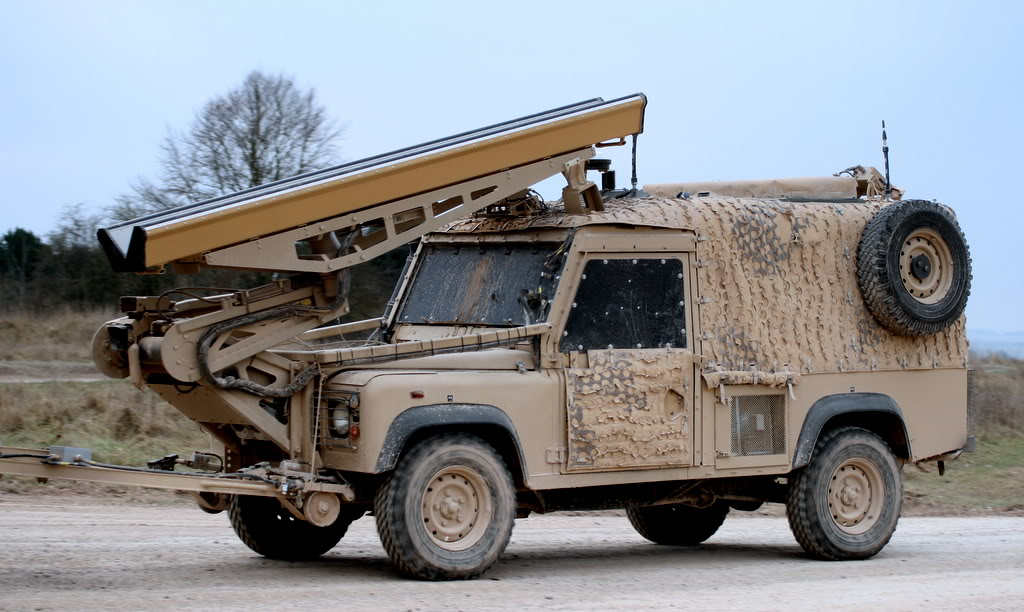
\includegraphics[height=0.25\textwidth]{2-Benchmarking/panama.jpg}} 
  & \subfloat[FORESIGHT RDV \parencite{canada2004}]{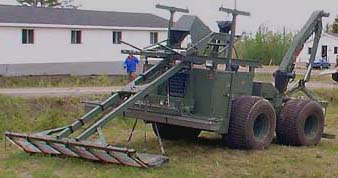
\includegraphics[height=0.25\textwidth]{2-Benchmarking/foresight.jpg}}\\
  \multicolumn{2}{c}{\subfloat[NIITEK Minestalker \parencite{niitek2015}]{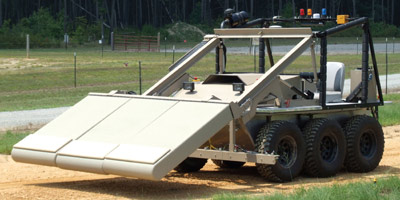
\includegraphics[height=0.25\textwidth]{2-Benchmarking/minestalker.jpg}}}
\end{tabular}}
\caption{Military and commercially available vehicles for landmine detection}
\figlabel{military}
\end{figure}
 
\Figref{military} shows three types of remotely controlled or autonomous landmine detection vehicles that have been used in military operations or are commercially available. 

\paragraph{PANAMA Snatch Land Rover}  The ``Snatch'' Land Rover was originally used as a lightly armoured transport vehicle by the UK, but was soon made redundant due to the increasing threat of improvised explosive devices (IEDs) \parencite{think2012}. The vehicle was then re-purposed as a low cost, unmanned solution to the IED problem \parencite{baxter2012}. Rather than using an expensive off-the-shelf device, the  expendable ``Snatch'' was modified to carry sensors including a GPR. The vehicles are usually deployed as part of a large team which handles demining, and are remotely operated.

\paragraph{General Dynamics FORESIGHT RDV} FORESIGHT is a multi-sensor landmine detection system, mounted on a vehicle that can be controlled remotely. The vehicle usually travels with a protection vehicle, which clears the the path ahead of surface-based devices, as well as mines just below the surface \parencite{canada2004}. The sensor suite consists of a GPR, minimum metal detector, which is used to detect small quantities of metal, and a infra-red camera \parencite{general2009}. A thermal neutron activation detector can also be added to directly detect explosives; this provide an added level of target confirmation.

\paragraph{NIITEK Minestalker} Develop by NIITEK, the Minestalker system utilises a high performance GPR and optional metal detector to detect a range of targets. The sensors are mounted on a vehicle which can be controlled remotely; the accompanying software system ensures that there is a high detection probability and a low number of false alarms \parencite{niitek2015}. Targets are marked both physically and with GPS, with a 1 metre resolution. 

\subsection{Research Vehicles}
Vehicles available for humanitarian landmine detection can be sorted into two categories, commercially available and research vehicles (\Figref{research}). The former are often smaller scale versions of similar devices used in the military, while the the latter are in development by research organisations, and are yet to be deployed.

\paragraph{Clearpath Husky} The Husky is an autonomous vehicle produced by Clearpath Robotics. A team at the University of Coimbra (Portugal) used this platform in 2012 to create a landmine detection vehicle \parencite{hennessey2014}. The sensor suite consists of a metal detector on a robotic arm, and a GPR. Unlike all the other vehicles introduced so far, the Husky has autonomous capabilities, meaning it can complete a mission without operator interaction \parencite{portugal2014}.

\paragraph{SILO6} SILO6 is a six-legged landmine detection robot. The six legs allow it to better traverse rough terrain, and increase mobility; in order to increase stability, the robot can lower its centre of gravity by bending its legs \parencite{santos2007}. The robot is semi-autonomous, however it has a limited sensor capability (metal detector sensing head).

\paragraph{tEODor} The tEDOor platform is commercially available for disposal of explosive ordnance. This platform was heavily modified by the Royal Military Academy (Belgium) to assist in humanitarian demining \parencite{cubber2014}. A metal detector array is fitted to the front of the platform, which can be controlled remotely. The system works in conjunction with an unmanned aerial vehicle, which firstly scans the area using visual and infra-red sensors, and identifies points of interest which tEODor investigates.   

\paragraph{Gryphon}
The Gryphon project is larger in scale than the rest of the research projects introduced. It uses a commercially available quad bike on which a large arm has been fitted \parencite{fukushima2008}. The length of the arm allows the vehicle to remain completely outside of the test lane, meaning this it is less susceptible to damage. A metal detector or GPR can be fitted to the end of the arm, though not at the same time.

\begin{figure}[ht]
\centerline{
\begin{tabular}{cc}
\subfloat[Clearpath Husky \parencite{hennessey2014}]{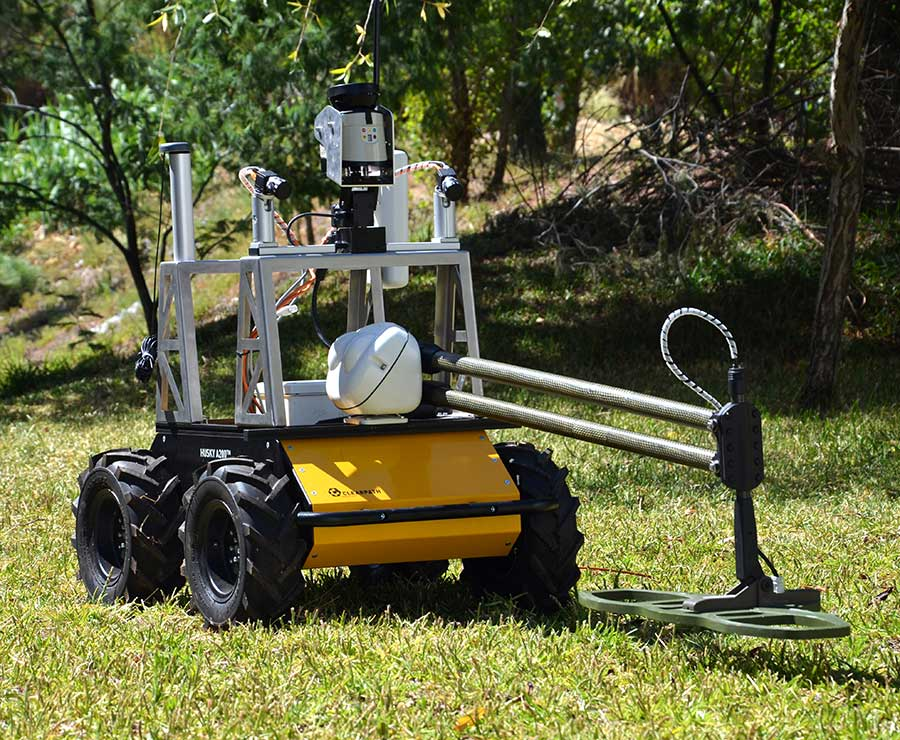
\includegraphics[height=0.3\textwidth]{2-Benchmarking/clearpath.jpg}} 
& \subfloat[SILO6 \parencite{santos2007}]{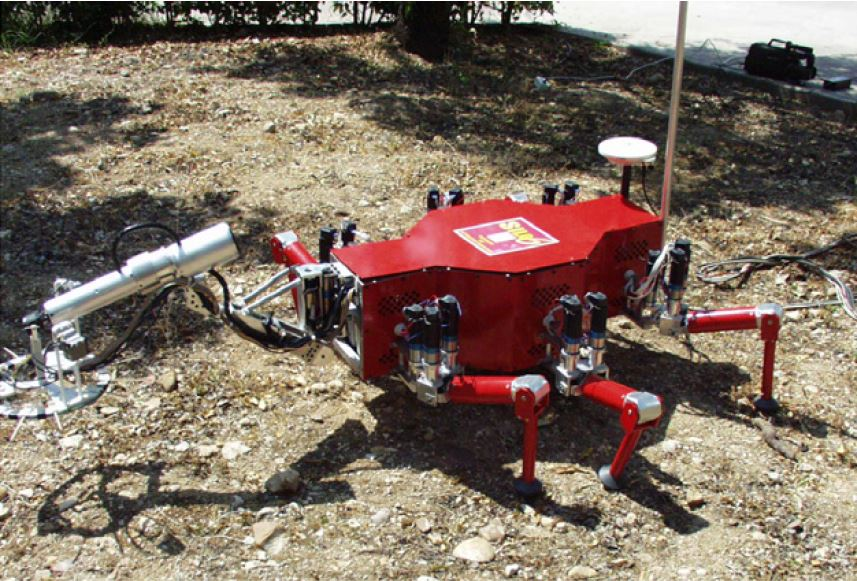
\includegraphics[height=0.3\textwidth]{2-Benchmarking/silo6.jpg}}\\
\subfloat[tEODor \parencite{cubber2014}]{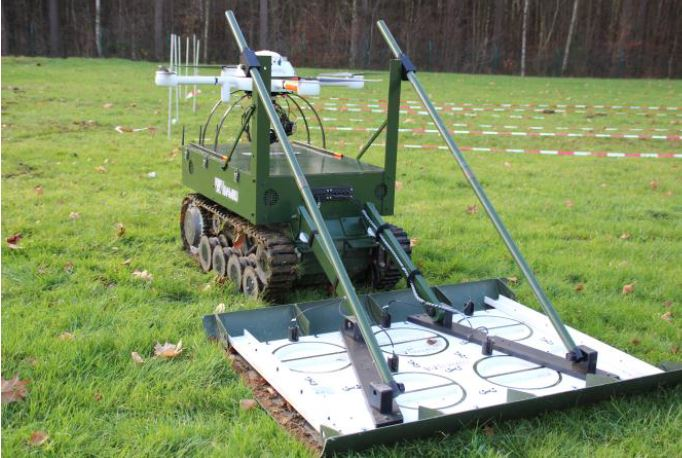
\includegraphics[height=0.3\textwidth]{2-Benchmarking/teodor.jpg}} 
& \subfloat[Gryphon \parencite{fukushima2008}]{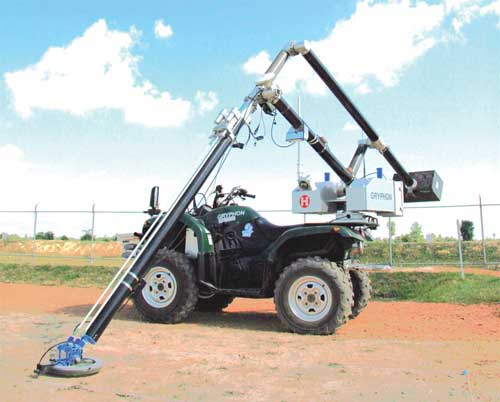
\includegraphics[height=0.3\textwidth]{2-Benchmarking/gryphon.jpg}}
\end{tabular}}
\caption{Research vehicles for landmine detection}
\figlabel{research}
\end{figure}

The various vehicles introduced show that there are many approaches to automated landmine detection, both in terms of the platforms used and the sensors available. While many solutions exist, no one method can be adapted to all scenarios, and there is much room for innovation and further research. 


\textcolor{blue}{RP wrote the parts below. Jono, just change. Cheers. }
\section{Landmine Detection}
\textcolor{red}{Make sure to refer to this goal for this benchmarking type}
%• Implementation of autonomous detection and classification of subsurface objects, with a focus on identifying objects with a high likelihood of being a landmine. interpretation of the output signals from the GPR and metal detector will be processed with the aim to identify and confirm with a percentage the likelihood of a threat. Supplied data sets will be used to create and tune 2 a detection algorithm to meet this goal, and operational trials will be conducted to test the effectiveness of the developed system.
%There have been similar projects that have used MD, GPR or a  combination of both to achieve detection and classification of landmines or unexploded ordinances (UXO). The various models of MD, GPR will be compared in order to determine if the specific details are suitable for landmine detection and if the scenario of operations (\textcolor{red}{insert reference to scenario of operations}) are achievable based on these specifications. 


\subsection{Metal Detectors}
\textcolor{red}{Insert some benchmarking here that Rahul did}

\subsection{Ground Penetrating Radar}
\textcolor{red}{Need to relate to the scope as well, i.e. soil types and operational environments\\}
% What has been achieved with the GPR in terms of the operation environment and soil types. etc. that can be linked and based on

%In order to meet the system requirements \textcolor{red}{(insert reference to system requirements here)} and  scenarios of operation of the landmine, there are operating parameters required. The operating specifications of a GPR for landmine detection are listed as follows \textcolor{red}{insert Pasolli reference here}:
% \begin{itemize}
% \item{\textbf{frequency:} 10 MHz - 3 GHz}
% \item{\textbf{Penetration depth:} 1 cm - 3 m.}
% \item{\textbf{Surface types:} Sand, humus soil}
% \item{\textbf{Operating time:} 1 ns to 60 ns}
% \item{\textbf{No. of data scans:} 200 - 600}
% \end{itemize}

%The following comparisons of specific GPRs that may be used in landmine detection should meet or exceed the specifications above. There are various types of commercial GPRs, such as NIITEK, SIRO-Pulse, and others as provided below. %-Still changing this part. 

%\paragraph{NIITEK GPR}
%AS provided in landmi
%\paragraph{SIRO-Pulse}

%\paragraph{DX Antenna Array GPR} This type of GPR meets the operating criteria above as specified in \textcolor{red}{see appendix}. There are various applications that this GPR may be used including archaeology,

%The detection of subsurface objects is one of the main uses for a GPR. This concept may be used in various applications including landmine detection. The GPR is able to detect landmines with various types of casing. An advantage of the GPR sensor is that there are both handheld and array types which assist in both manned and unmanned landmine detection operations. There are two types of GPRs, namely pulse radar (time-domain) and frequency-domain \textcolor{red}{specific reference here}. 

%In order detect and identify the subsurface objects as mentioned in \textcolor{red}{reference objective section}, the GPR signals are required to be processed. There are various methods implemented to detect landmines using GPR \textcolor{red}{INSERT CITE}. The first part is the preprocessing of the signals in order to remove signal clutter. This is processed further in order to identify the object under the surface and minimise false positives.

%The detection and classification of landmines and subsurface objects are achieved through existing algorithms, such as, hough transformation, bayesian, feature extraction, kalman filters.   

%\textcolor{red}{NOTE: Need to mention anything commercialised here. Types of GPR used, and the operation frequency they used. The penetration depth etc. etc. Nothing too specific. Just how they've done it. Elaborate on the types in Literature review.} \textcolor{green}{perfect. this is exactly what i was going to put in here - i had a spreadsheet on the GoogleDrive with most of this data in it, but it seems to have gone walkabout}

% Need to check everything
%NOTE NO PHYSICAL MARKING OF THE LANDMINE
%It is also possible to detect the composition of the explosives used in the landmines, however, this is only used in conjunction with the electromagnetic properties returned to receive the signals. 

%Link to Challenges in identifying the landmine due to background noise etc. 
% Need to mention that a database for identification is generally difficult to achieve with regards to current mines. Limitation include that the objects have similar reflected signals, such as rocks vs composite landmines. 

% Need to talk about the usefulness of the GPR and landmine together. How they complement each other. 

%\subsection{Multisensor Systems}
% Link to challenges in integration 

%The current challenges with landmine detection, including further elaboration of each signal processing methods are \textcolor{red}{reference literature review section}. 

\end{document}